% RQ5 Results: Inter-DAO Cooperation

\subsection{Overview}

We present results from \experimentruns{} simulation runs across five cooperation scenarios.

\begin{table}[htbp]
\centering
\caption{RQ5 Results Overview (Experiment 07)}
\label{tab:rq5-overview}
\begin{tabular}{lr}
\toprule
Parameter & Value \\
\midrule
Cooperation scenarios & 5 \\
Runs per scenario & 60 \\
Total simulation runs & 300 \\
\bottomrule
\end{tabular}
\end{table}

\subsection{Cooperation Success by Scenario}

\begin{figure}[htbp]
    \centering
    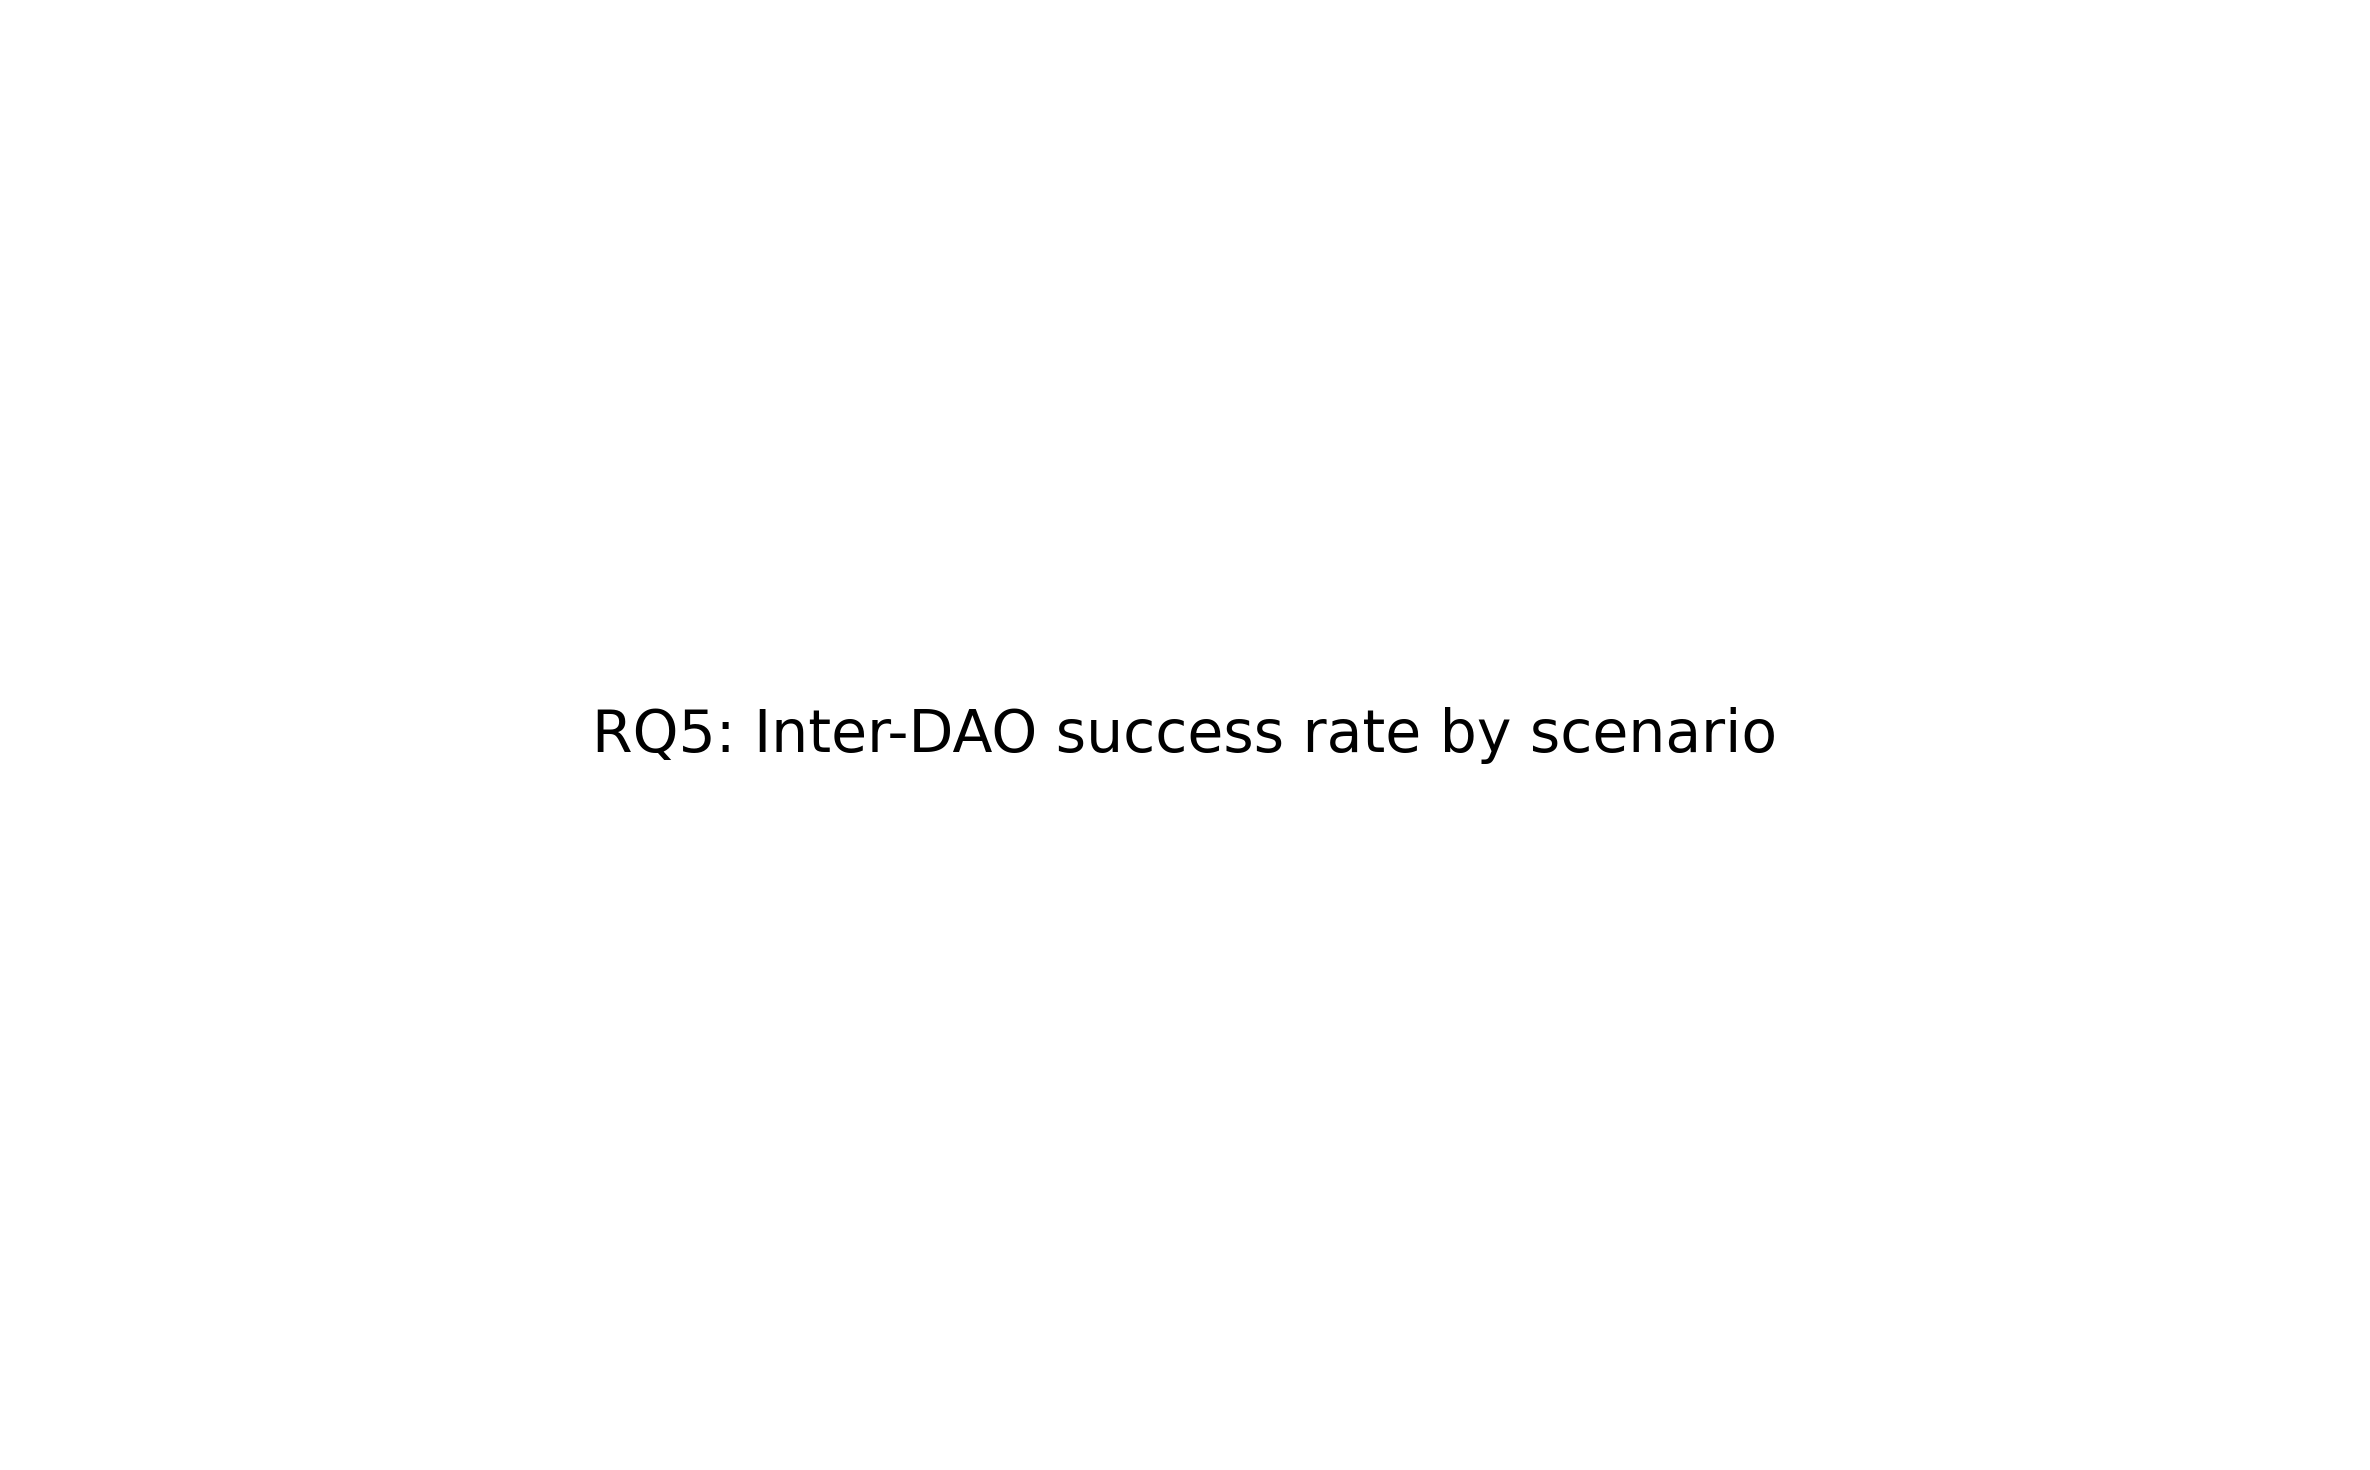
\includegraphics[width=0.8\textwidth]{../figures/rq5_success}
    \caption{Inter-DAO proposal success rate by cooperation scenario. Homogeneous DAOs achieve highest success rates; competitive scenarios show lowest cooperation.}
    \label{fig:rq5-success}
\end{figure}

\begin{table}[htbp]
\centering
\caption{Cooperation outcomes by scenario}
\label{tab:rq5-scenarios}
\begin{tabular}{lcccc}
\toprule
Scenario & Success Rate & Surplus & Flow Volume & Alignment \\
\midrule
\pl{Homogeneous} & \pl{--} & \pl{--} & \pl{--} & \pl{--} \\
\pl{Heterogeneous} & \pl{--} & \pl{--} & \pl{--} & \pl{--} \\
\pl{Asymmetric} & \pl{--} & \pl{--} & \pl{--} & \pl{--} \\
\pl{Hub-Spoke} & \pl{--} & \pl{--} & \pl{--} & \pl{--} \\
\pl{Competitive} & \pl{--} & \pl{--} & \pl{--} & \pl{--} \\
\bottomrule
\end{tabular}
\end{table}

\subsection{Surplus Generation}

\subsubsection{Complementarity Effects}

\begin{figure}[htbp]
    \centering
    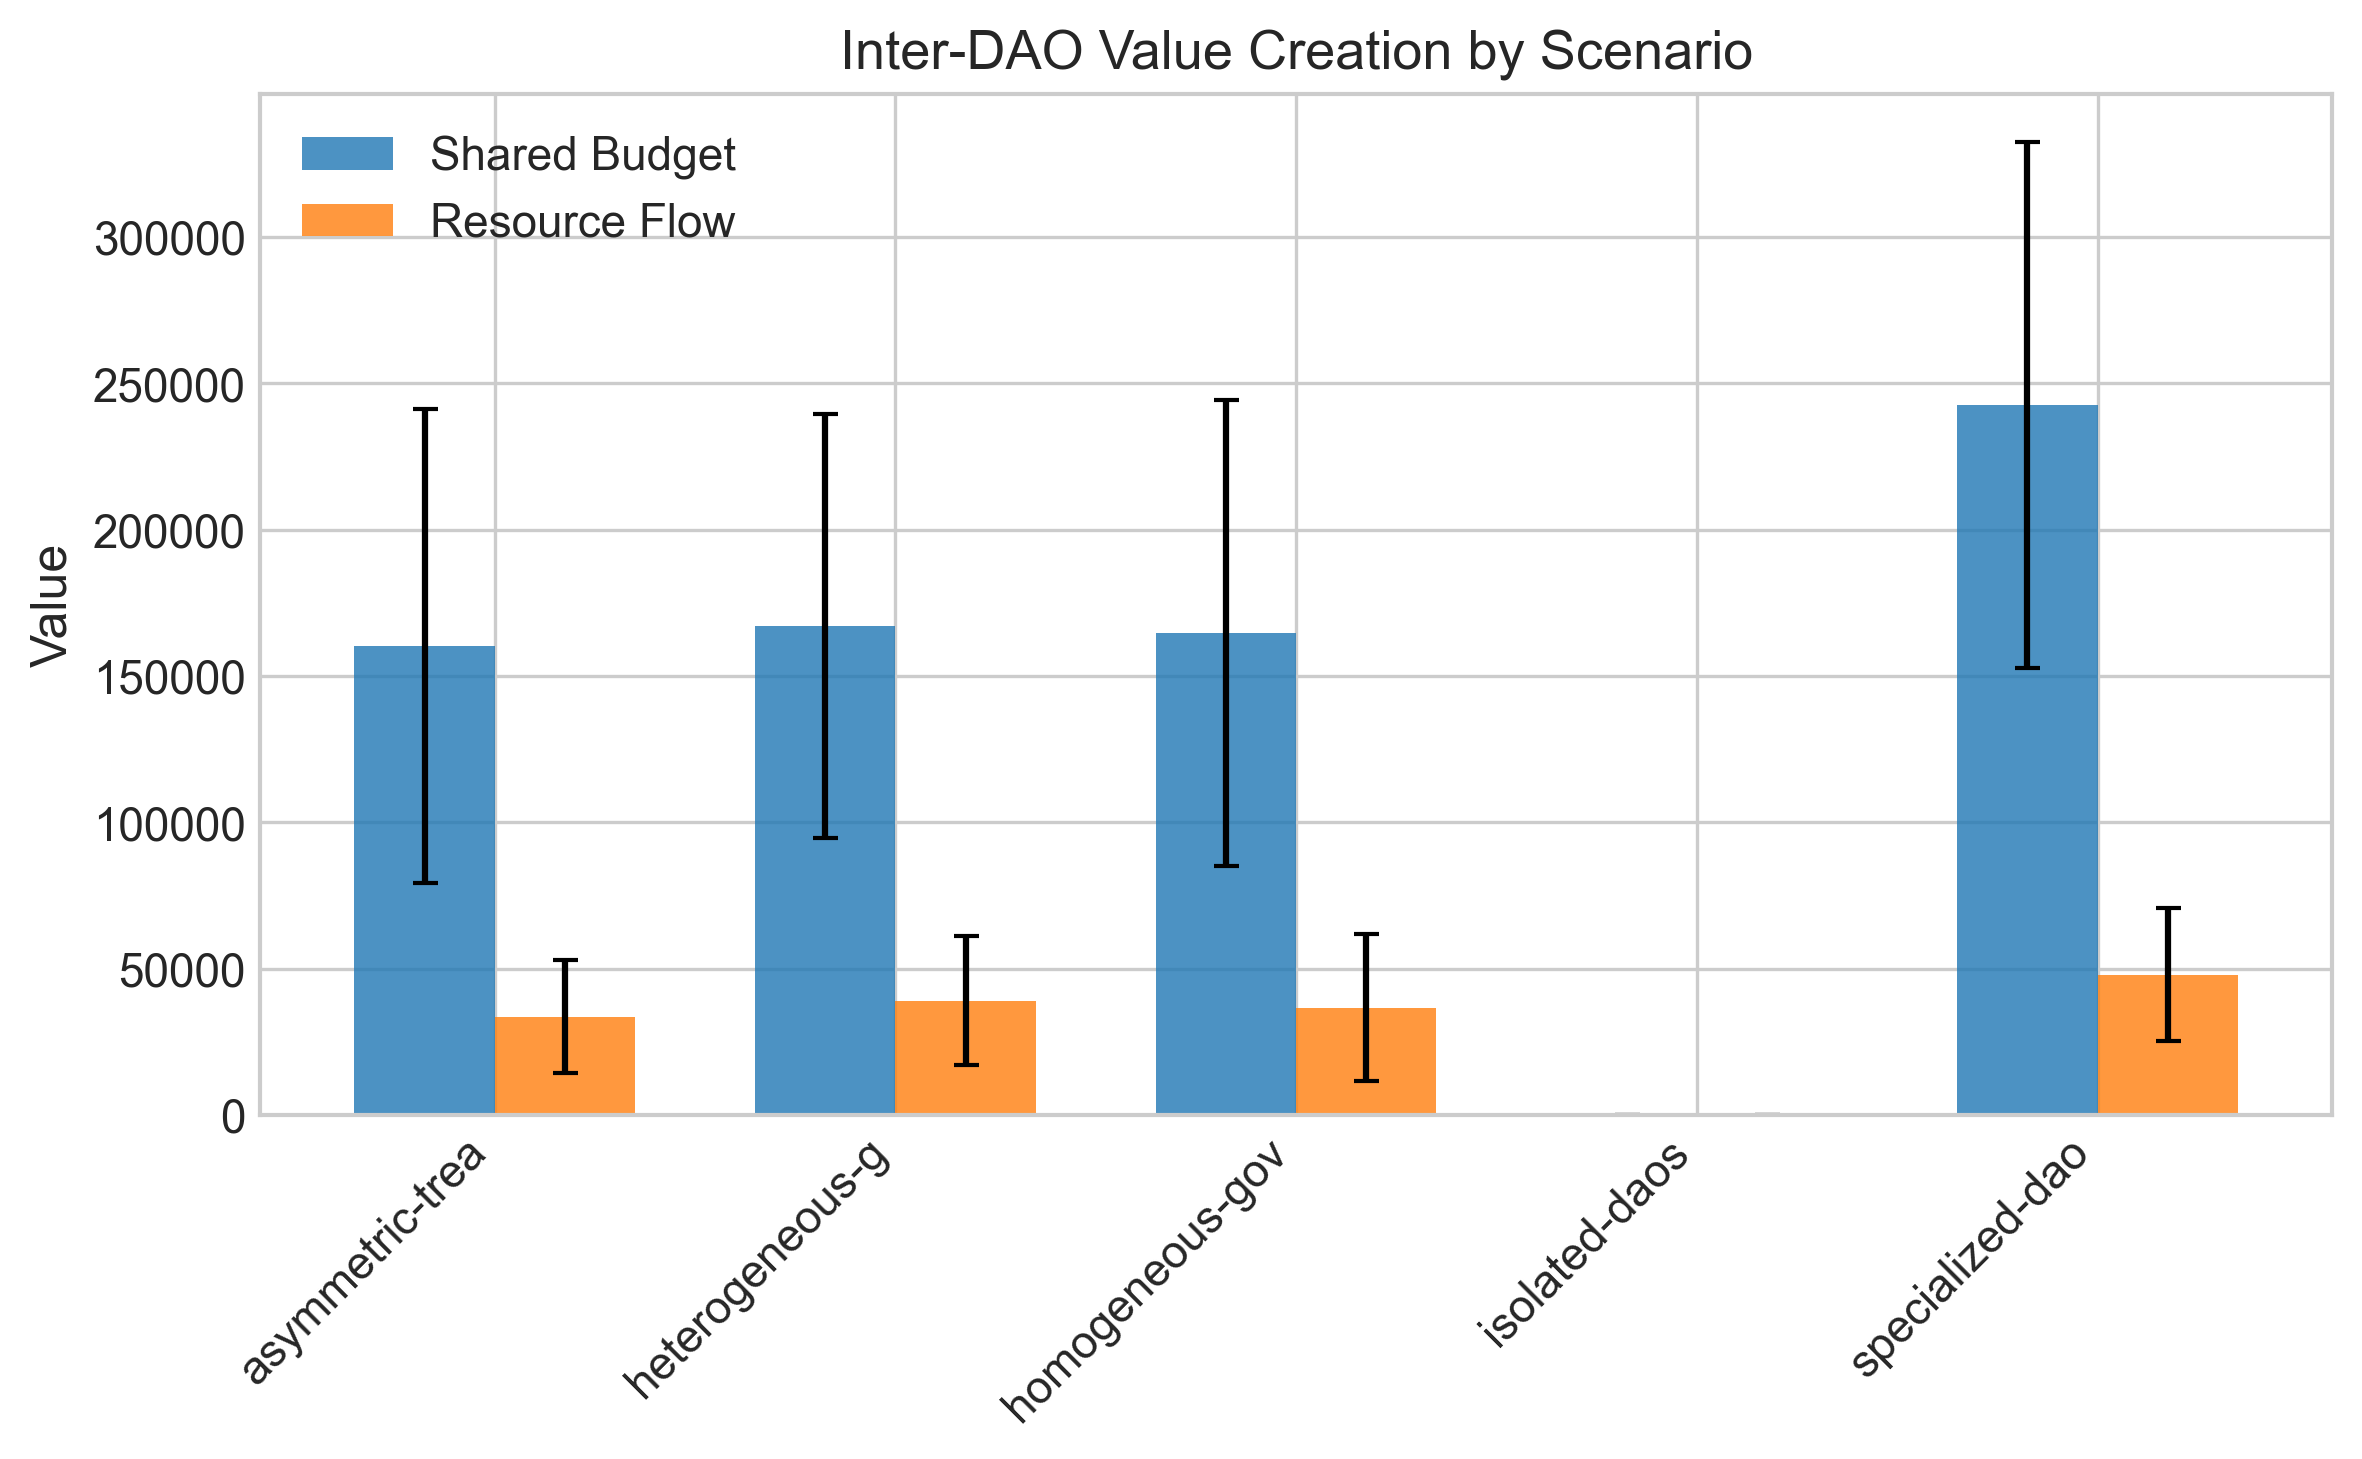
\includegraphics[width=0.8\textwidth]{../figures/rq5_surplus}
    \caption{Cooperation surplus by scenario. Heterogeneous DAOs generate largest surplus despite lower success rates, confirming complementarity effects.}
    \label{fig:rq5-surplus}
\end{figure}

\subsection{Fairness Mechanism Comparison}

\subsubsection{Asymmetric Scenario Analysis}

\begin{figure}[htbp]
    \centering
    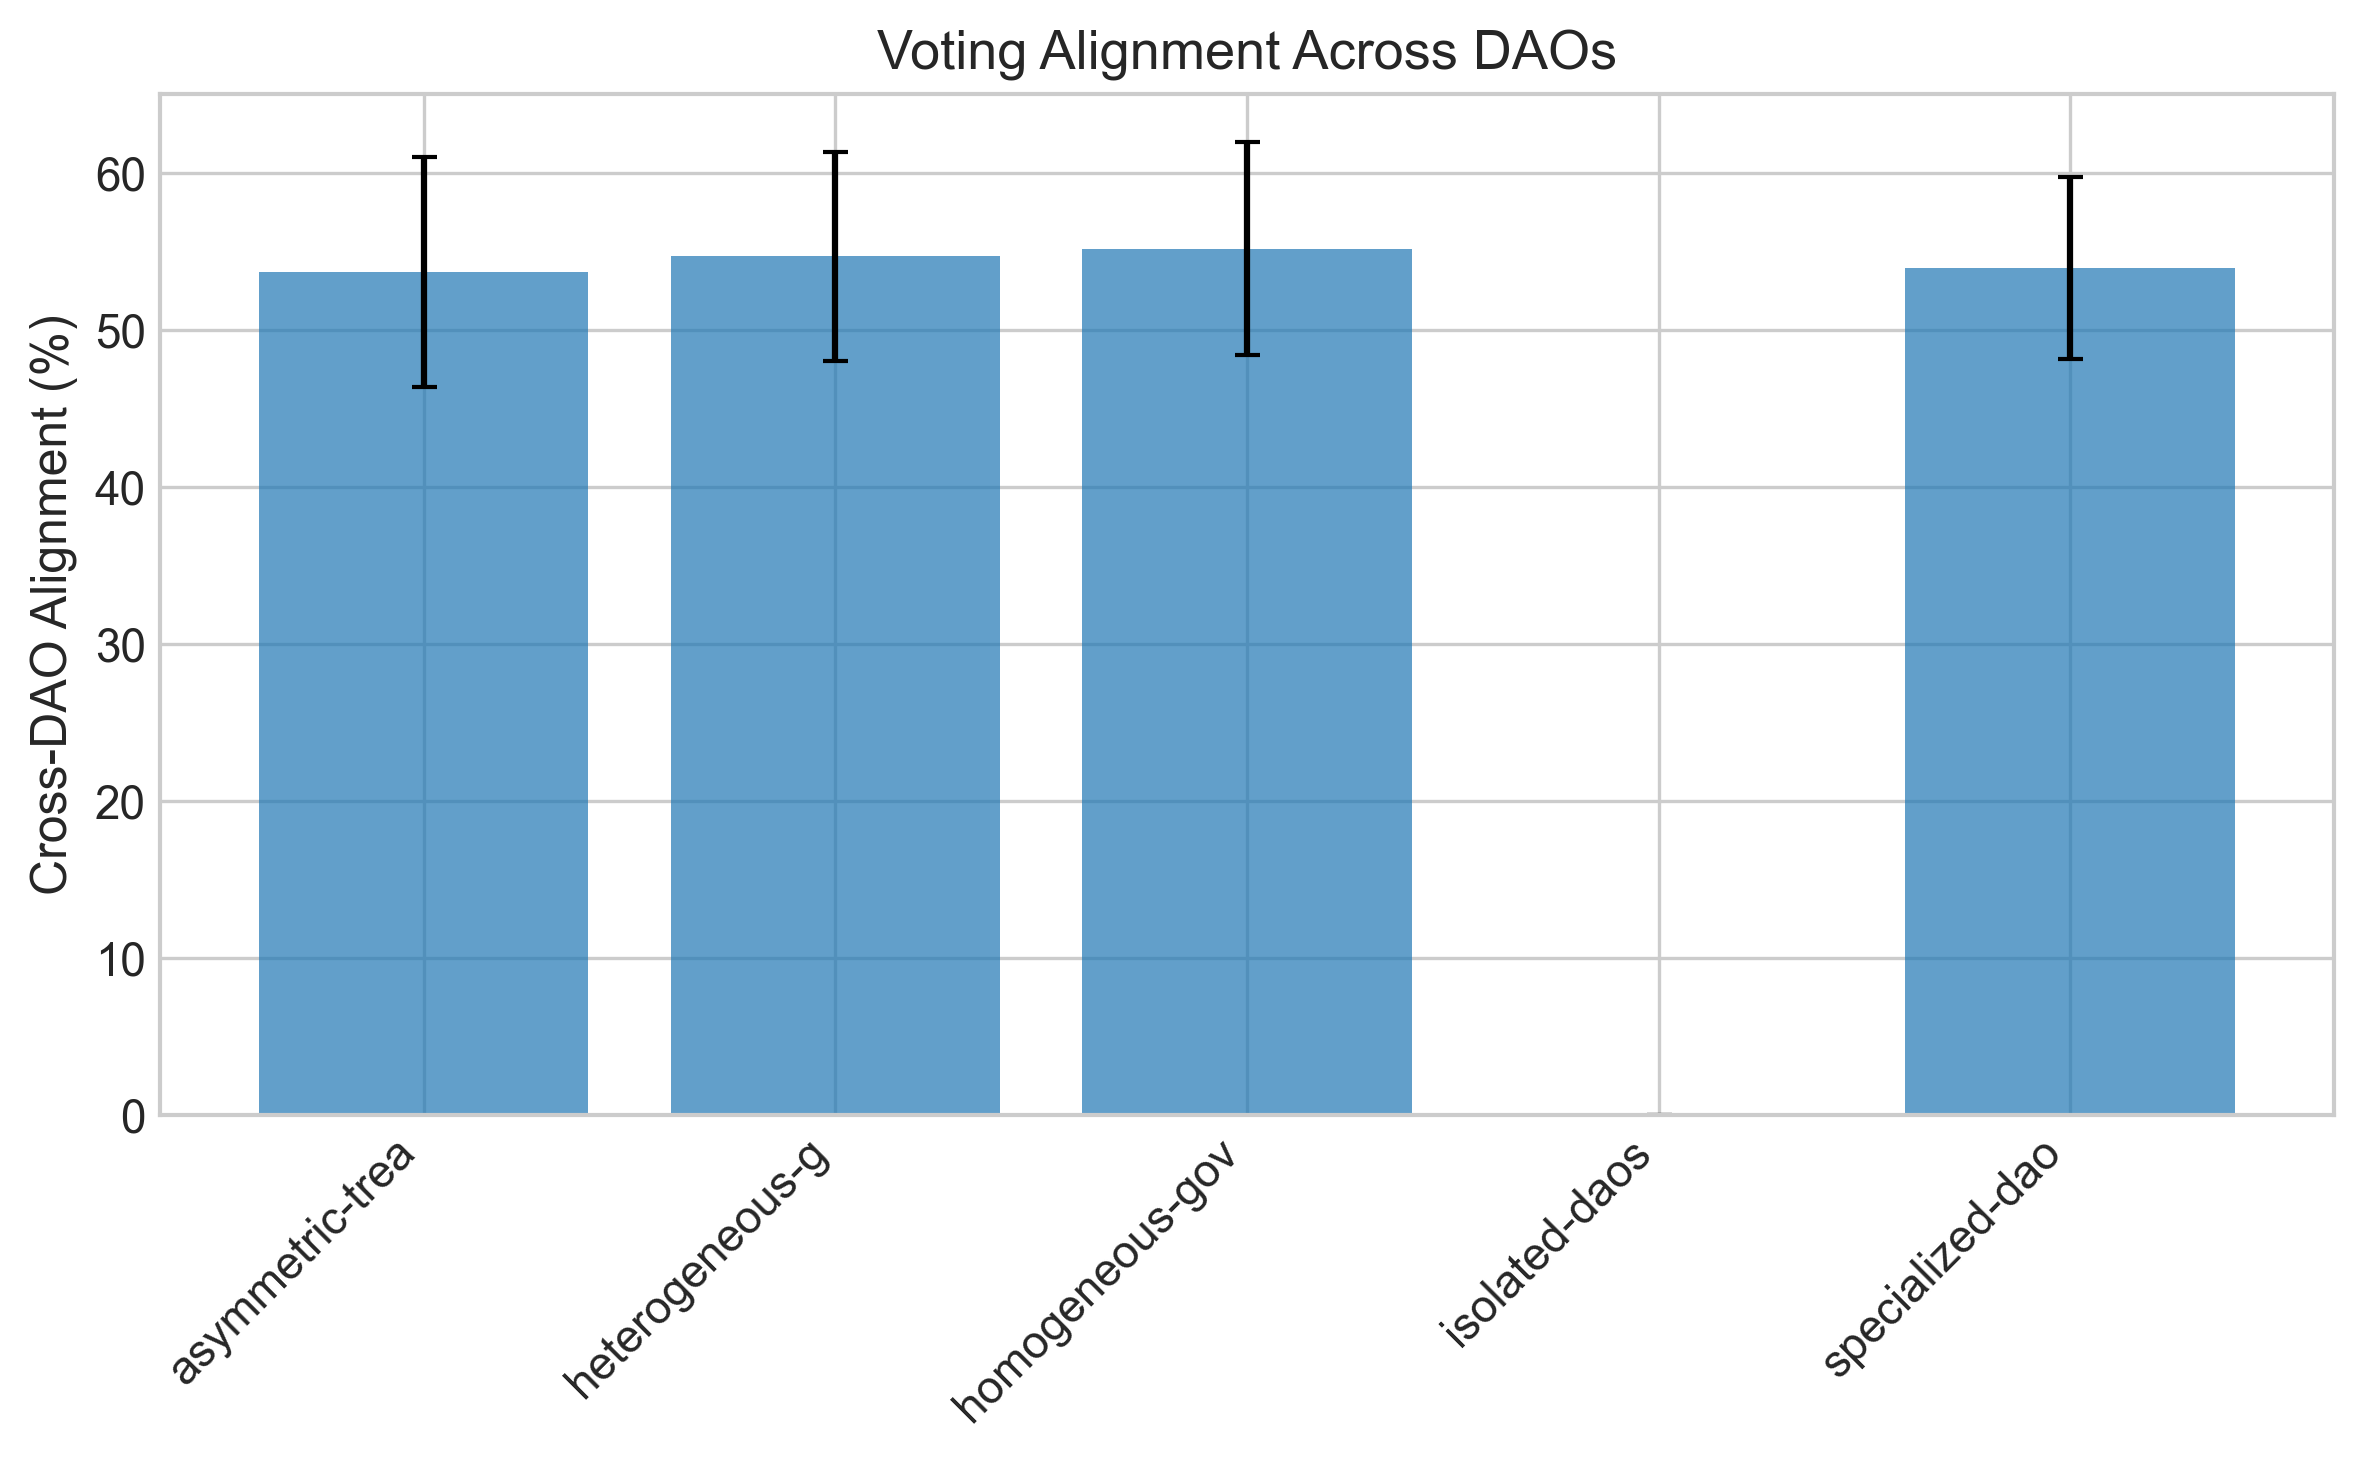
\includegraphics[width=0.8\textwidth]{../figures/rq5_fairness}
    \caption{Coalition stability under different fairness mechanisms in asymmetric scenario. Shapley division maintains longer cooperation than equal split.}
    \label{fig:rq5-fairness}
\end{figure}

\begin{table}[htbp]
\centering
\caption{Fairness mechanism comparison (asymmetric scenario)}
\label{tab:rq5-fairness}
\begin{tabular}{lccc}
\toprule
Mechanism & Coalition Duration & Small DAO Satisfaction & Success Rate \\
\midrule
\pl{Equal split} & \pl{--} & \pl{--} & \pl{--} \\
\pl{Shapley} & \pl{--} & \pl{--} & \pl{--} \\
\pl{Proportional} & \pl{--} & \pl{--} & \pl{--} \\
\bottomrule
\end{tabular}
\end{table}

\subsection{Hub-Spoke Coordination}

\begin{figure}[htbp]
    \centering
    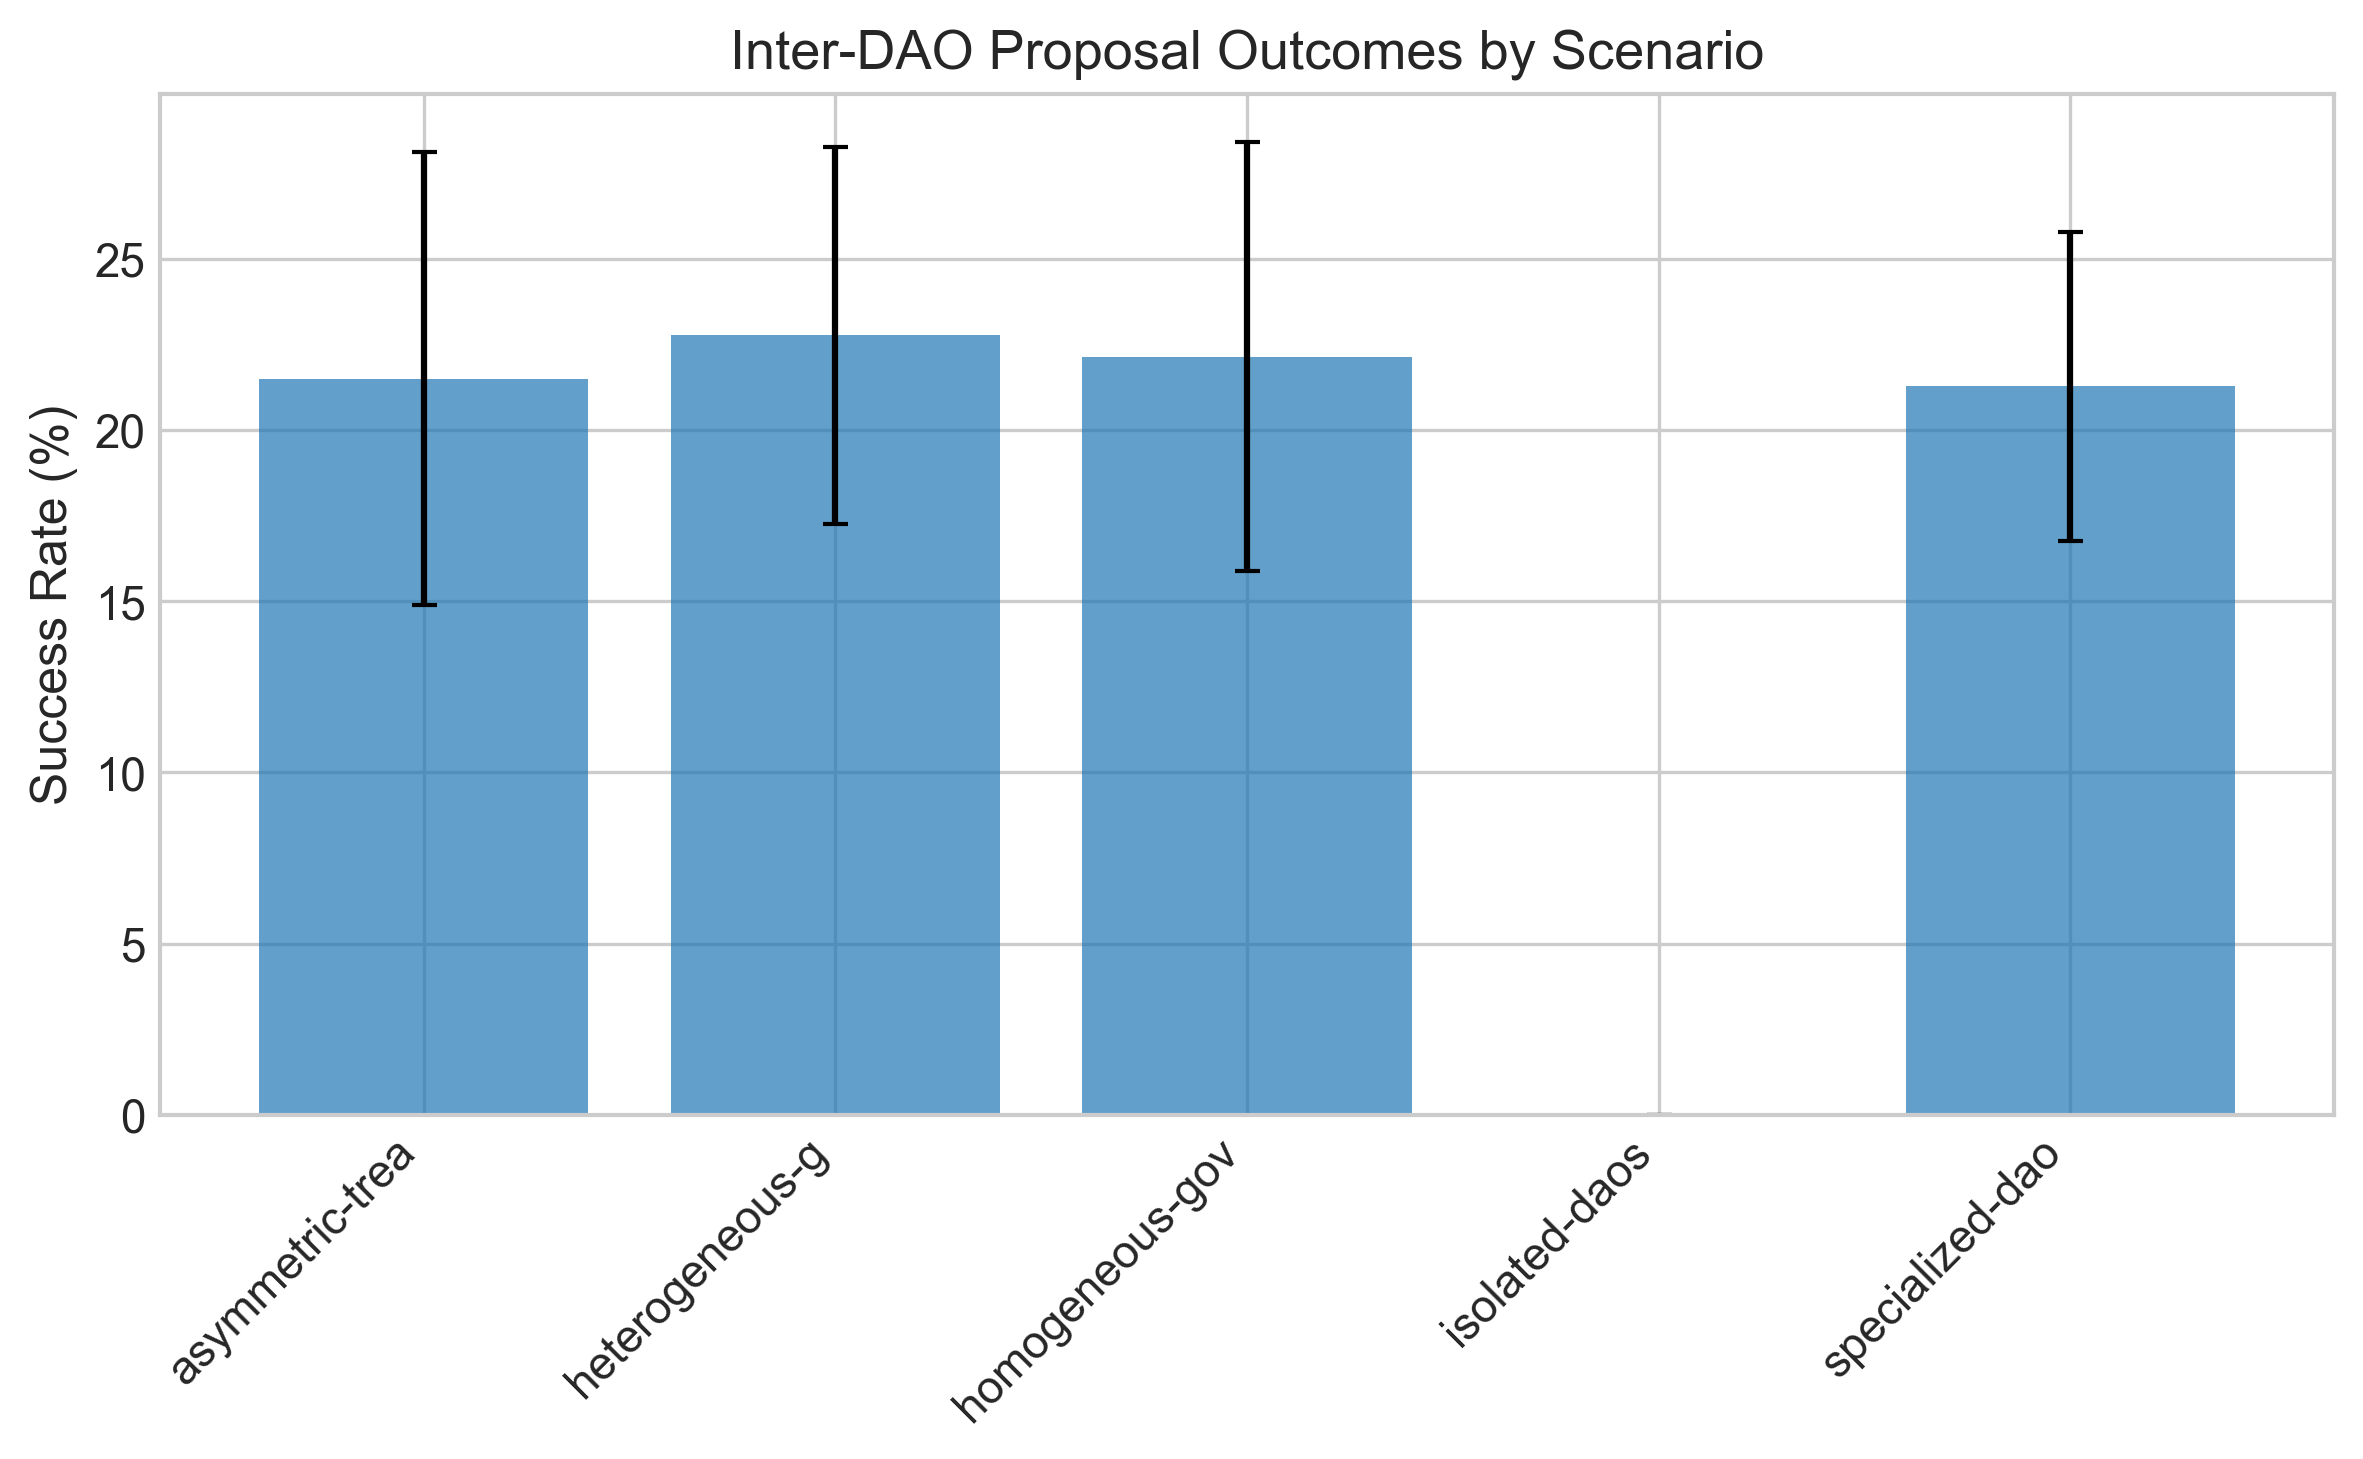
\includegraphics[width=0.8\textwidth]{../figures/rq5_hub}
    \caption{Coordination efficiency in hub-spoke vs. peer-to-peer structures. Hub coordination reduces time-to-agreement and increases multi-party proposal success.}
    \label{fig:rq5-hub}
\end{figure}

\subsection{Membership Overlap Effects}

\begin{figure}[htbp]
    \centering
    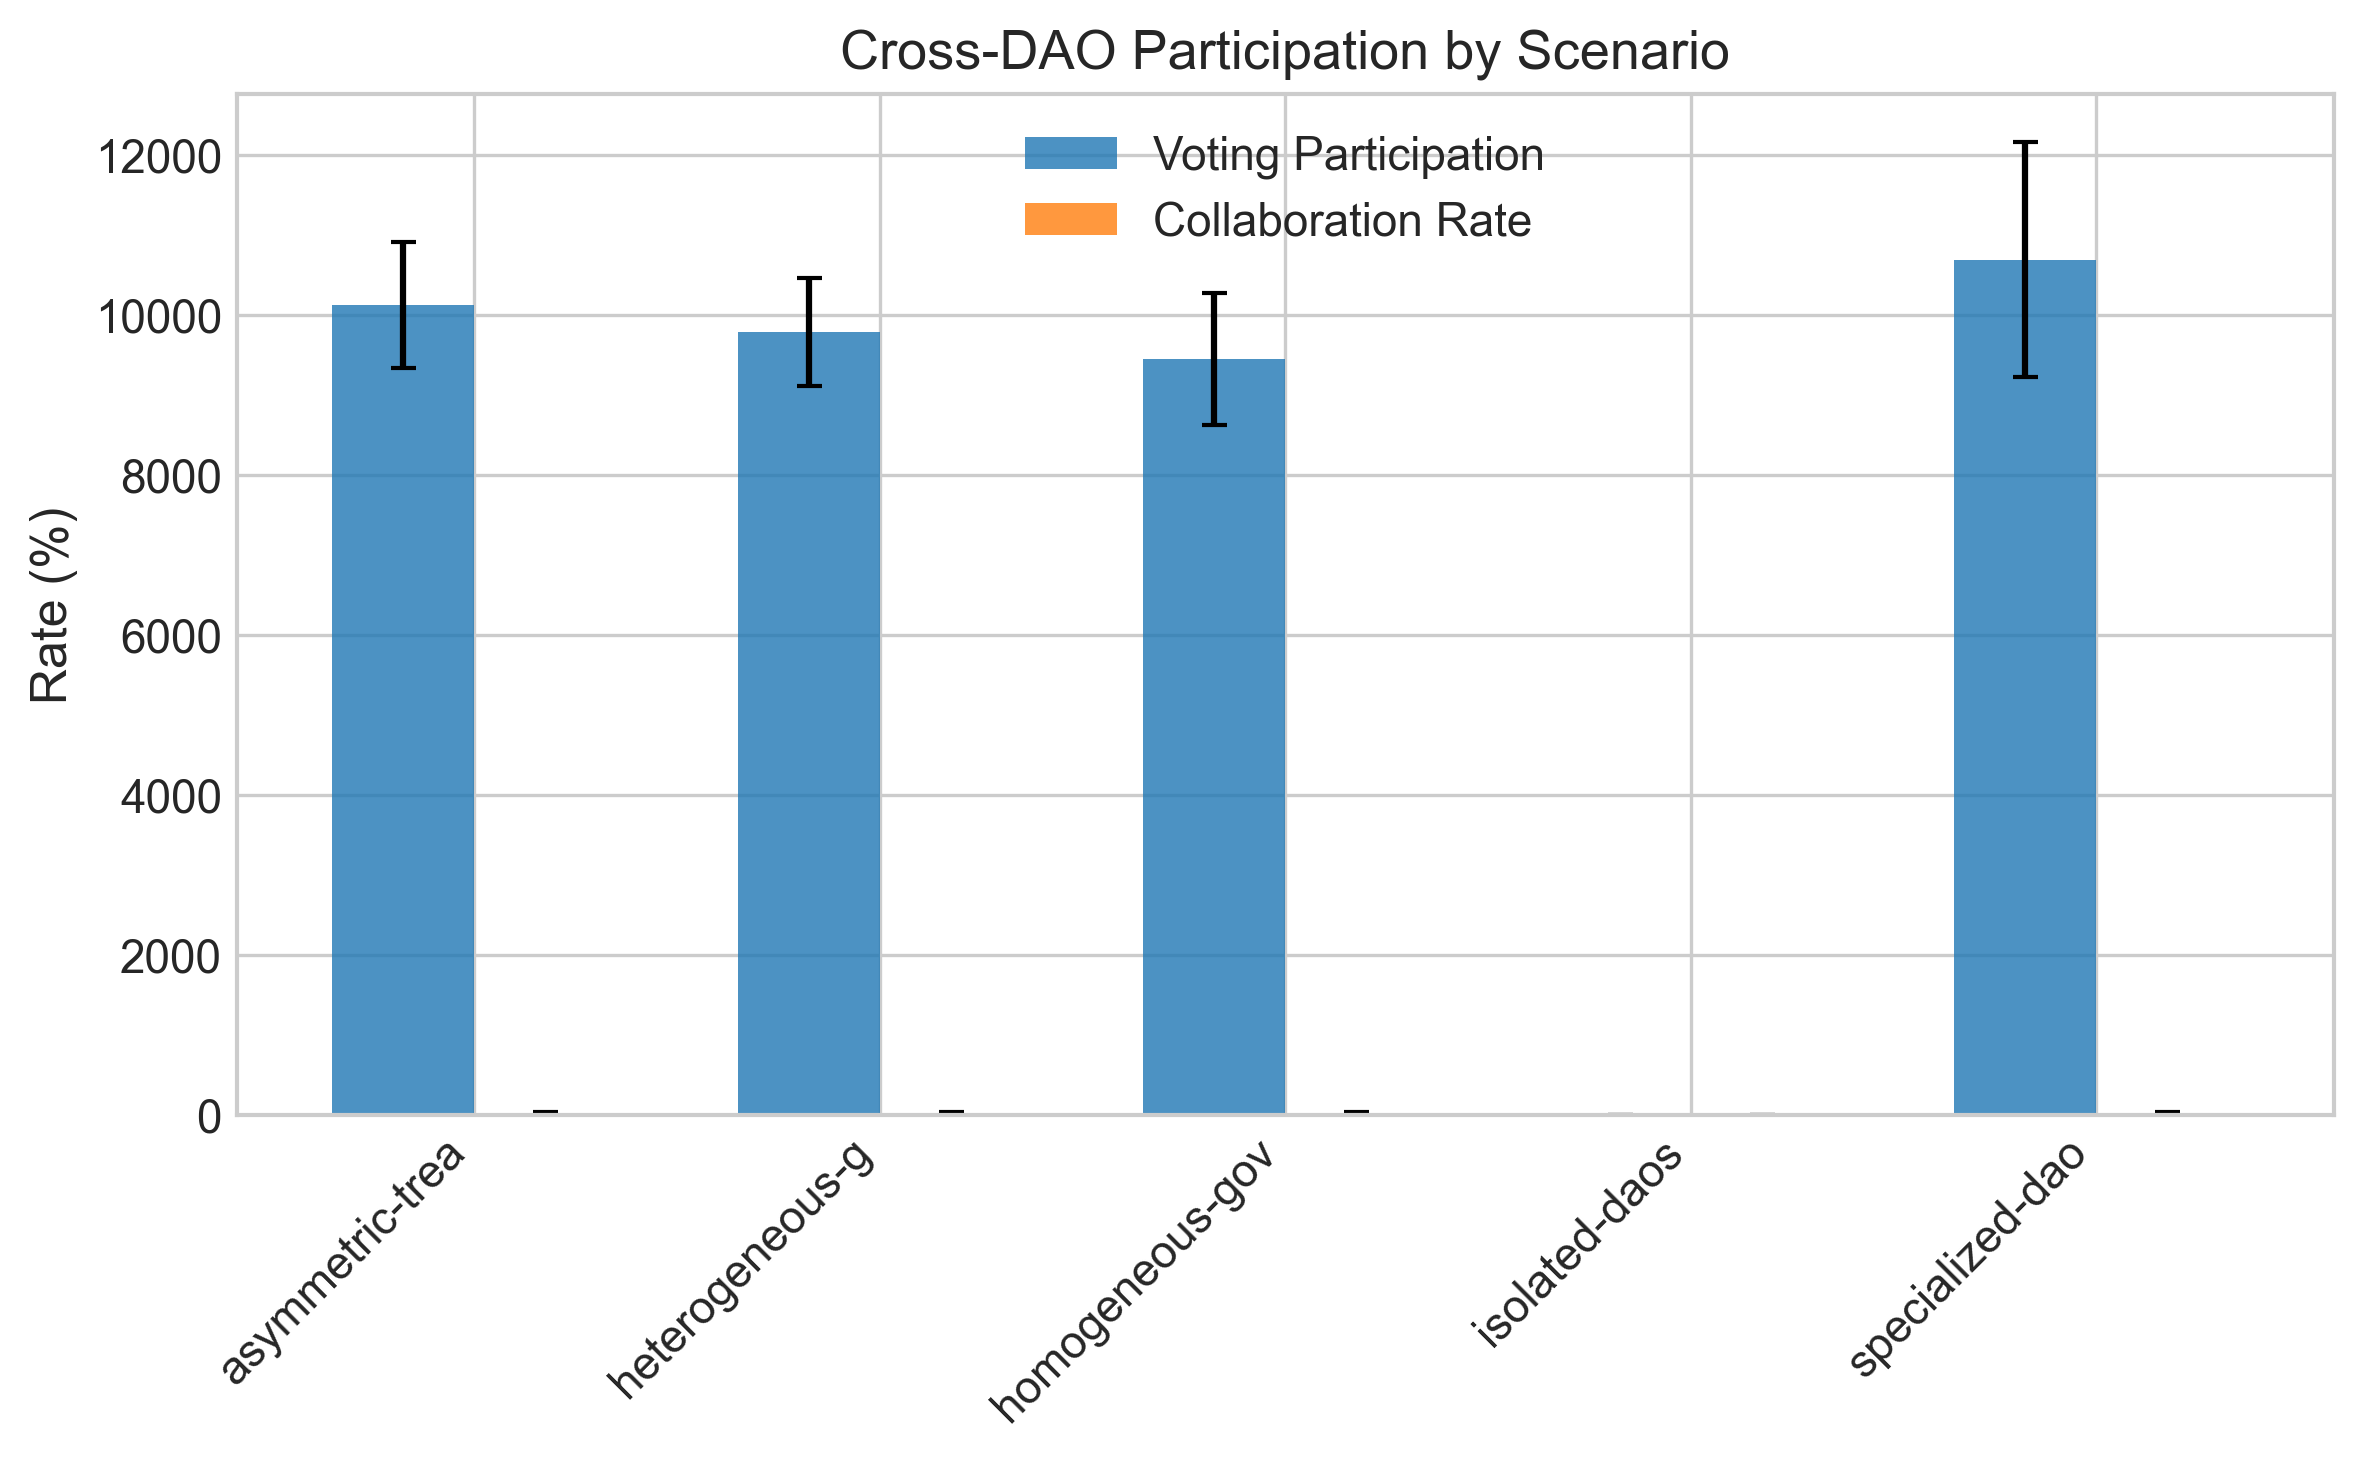
\includegraphics[width=0.8\textwidth]{../figures/rq5_overlap}
    \caption{Cooperation success rate vs. membership overlap. Cross-DAO token holders significantly increase cooperation probability.}
    \label{fig:rq5-overlap}
\end{figure}

\begin{table}[htbp]
\centering
\caption{Membership overlap effects}
\label{tab:rq5-overlap}
\begin{tabular}{lccc}
\toprule
Overlap Level & Success Rate & Alignment Score & Conflict Rate \\
\midrule
\pl{0-10\%} & \pl{--} & \pl{--} & \pl{--} \\
\pl{10-20\%} & \pl{--} & \pl{--} & \pl{--} \\
\pl{20-30\%} & \pl{--} & \pl{--} & \pl{--} \\
\bottomrule
\end{tabular}
\end{table}

\subsection{Hypothesis Evaluation}

\begin{table}[htbp]
\centering
\caption{Hypothesis testing results}
\label{tab:rq5-hypotheses}
\begin{tabular}{llcc}
\toprule
Hypothesis & Test & $p$-value & Result \\
\midrule
H5.1: Homogeneous $\rightarrow$ higher success & ANOVA & \pl{--} & \pl{TBD} \\
H5.2: Heterogeneous $\rightarrow$ larger surplus & t-test & \pl{--} & \pl{TBD} \\
H5.3: Asymmetric needs fairness & Comparison & \pl{--} & \pl{TBD} \\
H5.4: Hub improves coordination & t-test & \pl{--} & \pl{TBD} \\
H5.5: Overlap increases cooperation & Regression & \pl{--} & \pl{TBD} \\
\bottomrule
\end{tabular}
\end{table}

\subsection{Key Findings}

\begin{enumerate}
    \item \textbf{Success-surplus tradeoff}: Homogeneous DAOs cooperate more easily but generate less value; heterogeneous coalitions are harder to form but more valuable

    \item \textbf{Fairness enables asymmetric cooperation}: Shapley division or similar mechanisms are essential for stable large-small DAO partnerships

    \item \textbf{Hub structures improve multi-party coordination}: Central coordinators reduce negotiation costs and increase proposal success

    \item \textbf{Overlapping membership facilitates cooperation}: Cross-DAO token holders create natural alignment and trust channels

    \item \textbf{Competition limits but doesn't prevent cooperation}: Even rival DAOs can cooperate on clear public goods
\end{enumerate}
